\section{A primer on elevator systems}
\label{sec:elevators}

Elevator systems are characterized by different lifting mechanisms, 
e.g., hydraulic cylinders or electric motors, and different setups,
e.g., one or two cylinders, presence or absence of counterweights, and
dedicated machine room versus machine-room-less implements. In this
paper, we focus on Roped Hydraulic Elevators (RHEs), in which the
lifting power is provided by hydraulics. In Fig.~\ref{img:planView}
we show the cross-section of a RHE similar to those produced by
\liftcreate{}. Note that the image has been modified by removing 
some parts while enhancing others to ease understanding by a 
non-technical audience. The plan view accounts for the main components 
to be found in the design of an elevator. In the figure, the 
\textit{shaft} denotes the enclosure space in which the elevator 
is installed. Inside the shaft, we can observe the \textit{hydraulic
	cylinder}, providing lifting power, and  the \textit{car} attached
to the \textit{car frame}, a mechanical structure that supports the 
car and connects it to the piston through \emph{ropes} (not visible
in the plan view).  
The car frame slides within the shaft along the \textit{car rails}. 
The ropes are guided through a \textit{pulley} attached on top of the
piston: one end is secured to the shaft base, the other to the car frame.
Finally there are two kinds of doors, namely the \textit{car door} and
the  \textit{landing door}. As the name implies, the car door is only
one and it is attached to the car, while there is one matching landing
door for each floor.

\begin{figure}[t!]
	\caption{\label{img:planView} Cross-section (plan view) of a
		configured RHE. The shaft is the gray box surrounding the
		other components, the car frame is on the left side and
		doors at the bottom of the drawing.}
	\centering 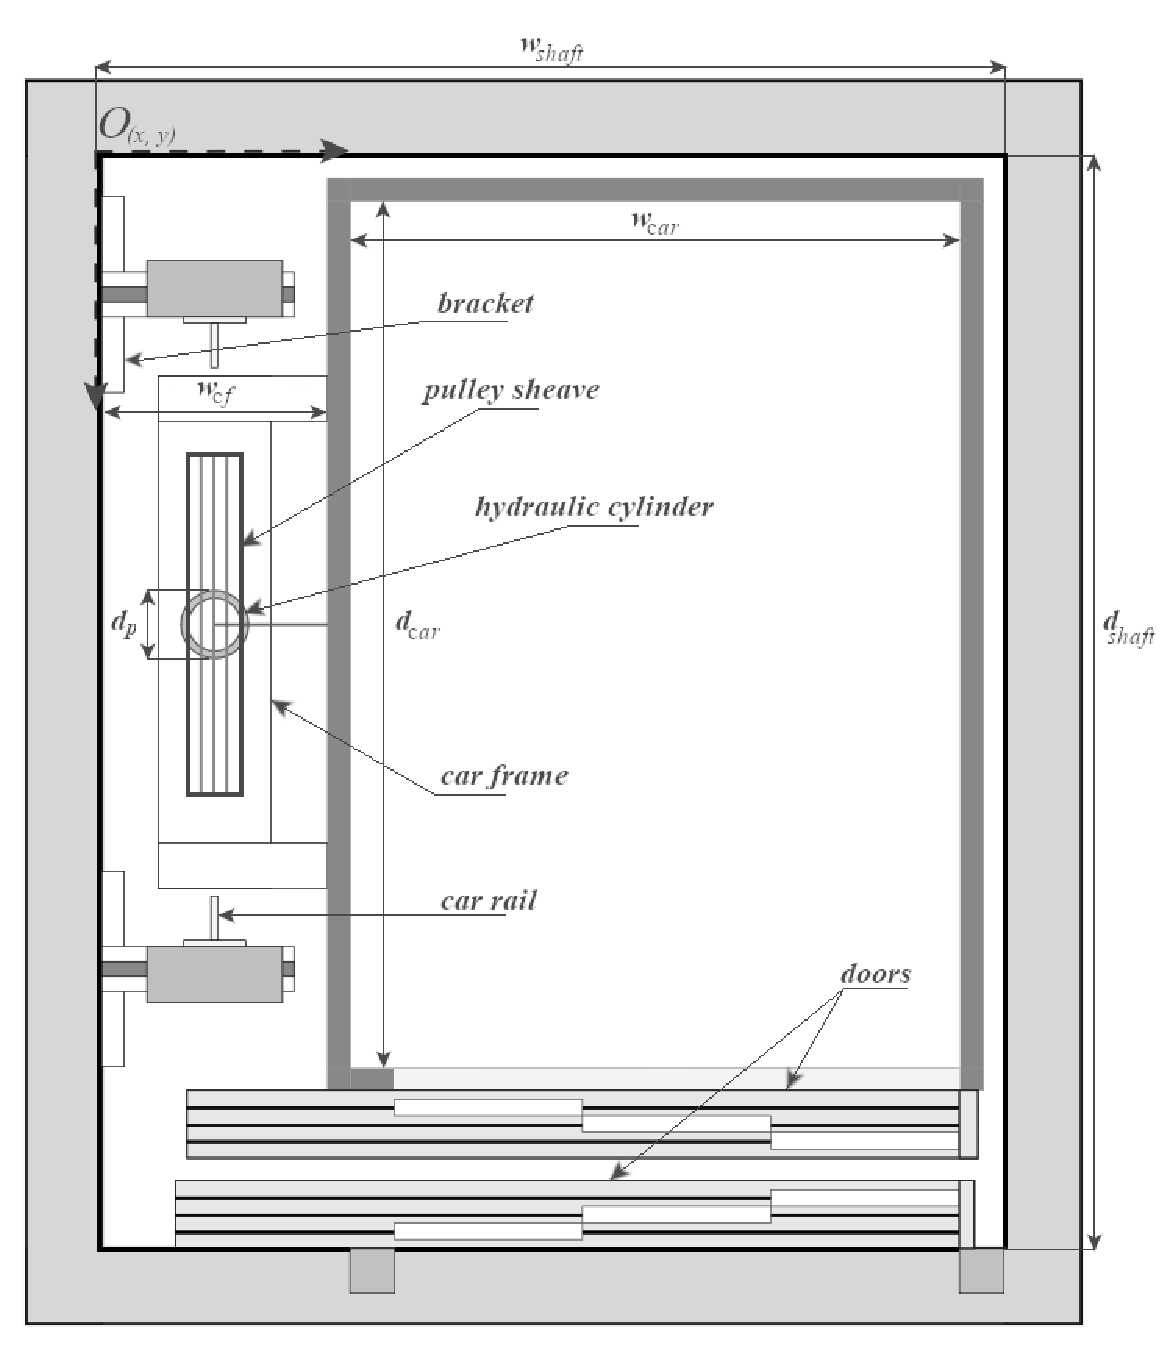
\includegraphics[width=.9\linewidth]{Elevator/planView.eps}
\end{figure}

Design of RHEs is usually performed in steps. The first one is the
choice of the doors and the car frame, whose positioning must be
determined considering shaft size, encumbrances, and tolerances since
a minimum distance between moving and fixed parts must always be taken
into account. In the second step, considering other parameters
like the distance between the car and the shaft or the materials used
for the car, an overall suspended weight and a maximum payload can
be computed. Based on these findings, other components like ropes,
rails, safety gear and the hydraulic cylinder can be engineered,
making sure that compliance to the norms and regulations is always
respected. In this phase, review of the previous phases might be
necessary because some choices might not result in feasible solutions,
which often makes the (manual) process to obtain the final design an
iterative trial-and-error endeavor. 
Considering the plan view of the of RHEs in Fig.\ref{img:planView}, 
in this work we  focus on elevators whose car frame is installed on the
left side and doors are installed at the bottom of the drawing. The
component selection we consider is limited to car frame, doors and
hydraulic cylinder, whereas placement involves car frame and doors.